\chapter{Algorithms and Approaches for Terrain LOD}
\section{Basics of Terrain LOD}
\subsection{Terrain Data Representation}
\subsubsection{Heightmaps}
One way of representing terrains is using \textit{heightmaps}.
A heightmap is a $n\times n$-grid that contains 
the height value $y$ for each $(x,z)$-position\footnote{We always denote $y$ for the up direction except if explicitly stated otherwise.}.
Positions are always spaced evenly in a grid-like manner,
but the distance between any two neighboring positions is variable.

The main advantage of heightmaps is that they allow for very simple storage and manipulation of height data, e.g. in form of images,
where low color values represent low areas of terrain and vice versa for
high color values. For a grayscale image, up to 256 height values can be used and for an RGB image,
more than 16 million height values are supported.
Looking up a height value for a given $(x,z)$-position is easy as well,
which consists of a simple lookup at the given position in the image.
Figure~\ref{fig:dom} shows a $2000 \times 2000$ heightmap of the mountain Dom in Valais, Switzerland.
\begin{figure}[H]
  \centering
  
\includegraphics[width=0.44\textwidth]{dom}
  \caption{$2000 \times 2000$ heightmap of the mountain Dom in Valais, Switzerland retrieved from SwissTopo \cite{alti3d}.}\label{fig:dom}
\end{figure}

\subsubsection{Triangulated Irregular Networks}
An alternative to the heightmap is the \textit{triangulated irregular network (TIN)} data structure.
A TIN consists of a collection of 3D vertices, where 
the arrangement of vertices can be irregular. Figure~\ref{fig:tin-example} shows 
an example of a TIN.
\begin{figure}[H]
  \centering
  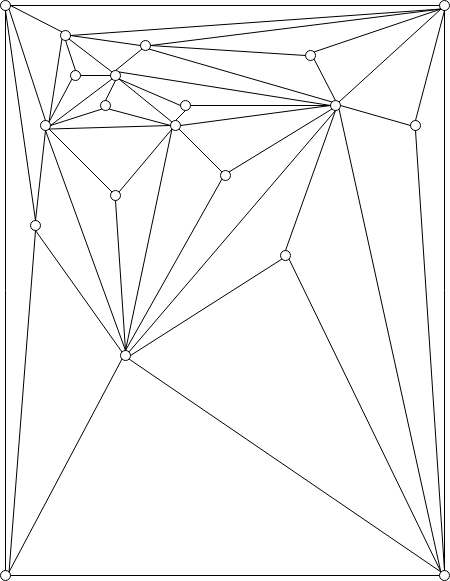
\includegraphics[width=0.52\textwidth]{tin-example}
  \caption{Example of a TIN. Note that the left area represents a terrain area with many changes 
  (e.g. mountains, hills, etc.), and the right area represents an area with few changes (e.g. flat areas).}\label{fig:tin-example}
\end{figure}

The main advantage of TINs is that fewer polygons need to be used for 
e.g. smooth terrain areas. Another advantage is that
special terrain features can be modelled 
which are usually difficult to model with heightmaps, such as overhangs, cliffs and caves, 
The disadvantage of TINs, however, is that the full $(x,y,z)$ coordinates need to be stored,
whereas with heightmaps, only the height value $y$ needs to be stored.

\subsection{Bintrees and Quadtrees}
\textit{Binary triangle trees (bintrees)} and \textit{quadtrees} are 
recursive data structures based on triangles and quads respectively.
A bintree consists of up to two child triangles, both of which in turn also consist of up to two child triangles each, and so on.
Quadtrees are structured similarly, with a quad consisting of up to four child quads, and each child quad consisting
of up to four child quads, and so on.
Figure~\ref{fig:bintree-quadtree-example} shows an example of a bintree and a quadtree.

\begin{figure}[H]
  \centering
  \subfloat[\centering]{{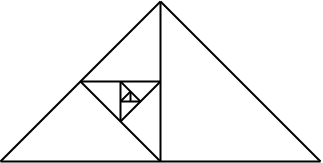
\includegraphics[width=0.43\textwidth]{bintree-example} }}
  \qquad
  \subfloat[\centering]{{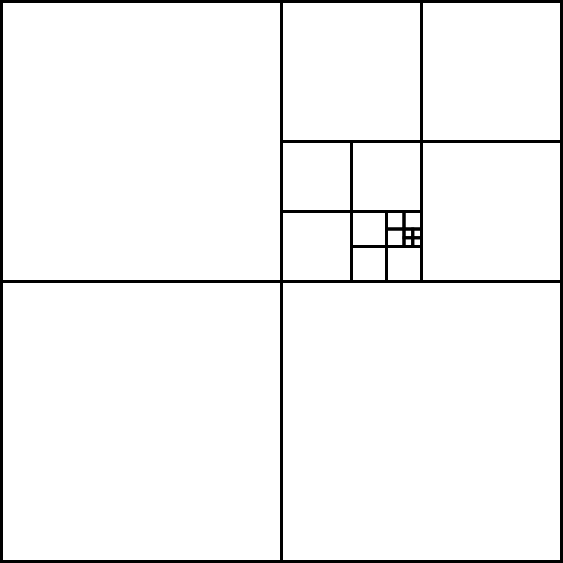
\includegraphics[width=0.33\textwidth]{quadtree-example.png} }}%
  \caption{Example of a bintree (a) and a quadtree (b).}\label{fig:bintree-quadtree-example}
\end{figure}

The main advantage of bintrees and quadtrees is that 
LOD can be modelled very naturally with them.
Bintree/quadtree sections with few children correspond to a low LOD and 
vice versa for bintree/quadtree sections with many children.

\subsection{Potential Problems During Terrain Rendering}
While terrain LOD algorithms dramatically improve the performance of terrain rendering, 
there are certain faults that can occur during rendering. 

\subsubsection{Cracks}
Cracks and holes in terrains can appear when a higher LOD terrain section is bordered 
by a lower LOD terrain section. The main problem is that when a vertex $v_{\text{high}}$ of a higher LOD terrain section lies on the edge $e_{\text{low}}$
of a lower LOD terrain section and the $y$ coordinate of $v_{\text{high}}$ is greater or less than the 
height of $e_{\text{low}}$ at that point, the difference in height causes the crack to appear, as shown in figure~\ref{fig:crack-example}.
\begin{figure}[H]
  \centering
  \subfloat[\centering The crack is caused by the height difference of $v_{\text{high}}$ and $e_{\text{low}}$.]{{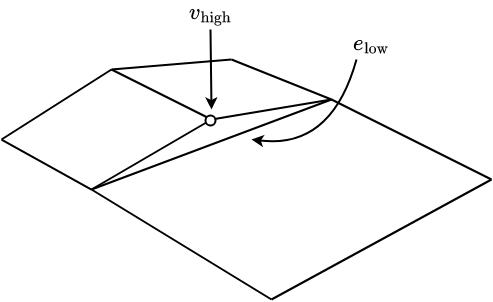
\includegraphics[width=0.5\textwidth]{crack-example} }}
  \qquad
  \subfloat[\centering The background color is set to red to highlight the cracks.]{{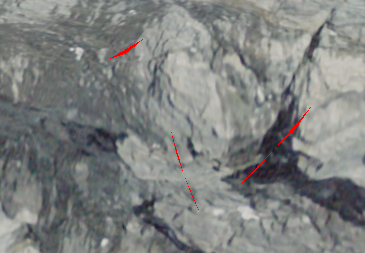
\includegraphics[width=0.4\textwidth]{cracks-terrain} }}%
  \caption{Illustration of a crack (a) and some examples of cracks in a real rendered terrain (b).}\label{fig:crack-example}
\end{figure}
Cracks can be solved by either of the following, depending on the capabilities of the LOD approach:
\begin{itemize}
  \item Removing the vertex in question, cuasing the higher and lower LOD meshes to be connected seamlessl (in figure~\ref{fig:crack-example} vertex $v_{\text{high}}$).
  \item Inserting an extra vertex at the border edge of the lower LOD mesh \cite[p.~194]{lodfor3dgraphics} (in figure~\ref{fig:crack-example} on top of vertex $v_{\text{high}}$). The disadvantage of this is that an extra vertex needs to get created.
  \item By force splitting the terrain mesh to get a more continuous mesh \cite[p.~193]{lodfor3dgraphics}. 
\end{itemize}

\subsubsection{Popping}
The phenomenon of \textit{popping} occurs when the camera is moving 
and the transition of the terrain's LOD level causes visual pops to appear.
Popping decreases the realism of the terrain and should be as minimal as possible.
Popping can be reduced by introducing \textit{vertex morphing} \cite{geomipmapping,geomclipmaps,cdlod}, 
i.e. by animating the transition of one LOD level to the next seamlessly through interpolation.

\section{ROAM}
\textit{ROAM} (short for \textbf{R}eal-time \textbf{O}ptimally \textbf{A}dapting \textbf{M}eshes) 
is a terrain LOD algorithm developed by Duchaineau \textit{et al.} \cite{roam} published in 1997.
ROAM represents the terrain mesh using bintrees and performs triangle splits and merges
for generating and removing detail. 
The splits and merges happen mainly on the CPU, which makes ROAM a mainly CPU-based approach.

\subsection{General Idea}
The central idea of the algorithm is to use temporal coherence: the mesh from a previous frame $\mathbf{T}_{f-1}$ is used to compute 
the mesh of the current frame $\mathbf{T}$, rather than building up the mesh from ground up for each frame.
This is done using two priority queues: a split queue $\mathcal{Q}_s$ and a merge queue $\mathcal{Q}_m$.
The split queue contains splittable triangles $T$
and the merge queue contains mergable triangle pairs $(T,T_B)$.
The elements of the priority queues are ordered by 
various geometric error metrics, which are explained in the subsection ``Error Metrics'' of this report.
At each frame, the terrain mesh gets split and merged using $\mathcal{Q}_s$ and $\mathcal{Q}_m$. until either the required size/accuracy is reached
or the time runs out.
ROAM is designed as a greedy algorithm, meaning it will always performs the most optimal splits/merges for each frame.

\subsection{Error Metrics}
The original ROAM paper mentions various error metrics for the priority queue ordering,
which are explained in the following paragraphs.

\paragraph{Wedgies} \textit{Wedgies} are nested bounding volumes around triangles that are computed 
while building the initial mesh at the beginning of the algorithm.
A wedgie is defined to contain the entire $x$ and $z$ extent\footnote{The original ROAM paper uses $z$ for the up direction. For the sake of consistency with the rest of this report, we will use $y$ as the up direction here.}
of a triangle and the height $y$ including some additional space above and below the highest and lowest points,
respectively.

\paragraph{Geometric Screen Distortion}
Another metric is the distance between where a node is supposed to be on the screen and where the algorithm placed the node.
The maximum of all distances is calculated and used as the base priority metric of the algorithm.

\subsection{Other Optimizations}
\paragraph{View-frustum Culling}
An optimization that is mentioned is view-frustum culling. In each frame, various flags are updated during 
the recursive traversal of the bintree. These flags indicate whether a wedgie is inside the view-frustum 
fully, partially, or not at all.

\paragraph{Incremental Triangle Stripping}
The ROAM paper reports using \textit{incremental triangle stripping} for optimizing the performance of the rendering.
This is simply refers to using triangle strips for rendering. which is supported by all major graphics APIs.

\subsection{Conclusion}
The runtime of ROAM is independent of the screen resolution and is proportional to the 
number of triangle changes per frame. 

%\section{Röttger's Quadtree-based Algorithm}
%TODO

\section{GeoMipMapping}
\textit{Geometrical Mipmapping (GeoMipMapping)} is a terrain LOD approach developed by de Boer \cite{geomipmapping} in the year 2000. 
It applies the idea of texture mipmapping to terrain rendering.

\subsection{General Idea}
The central idea of GeoMipMapping is its analogy to texture mipmapping: just like how textures of far away objects are rendered using lower resolution texture mipmaps,
terrain areas that are far away from the camera should also be rendered with a lower resolution mesh.

This is achieved by splitting up the terrain into so-called \textit{blocks} (also called \textit{patches}) of a fixed width $2^n + 1$ for an arbitrary $n \in \mathbb{N}$.
Each block has a LOD level\footnote{The original GeoMipMapping paper uses 0 to denote the maximum LOD level and vice-versa for the minimum LOD level. In order to avoid any confusion with the term \textit{LOD}, this report denotes 0 as the minimum LOD level and vice versa for the maximum LOD level.} $0\leq l \leq n$ that changes dynamically at runtime.
At load time, every block is computed at every LOD level and subsequently stored, e.g. on an index buffer.
Each such representation of a block at a specific LOD level is called a \textit{GeoMipMap}.
For each GeoMipMap, the number of vertices on one side is $2^{l}+1$ and the number of quads is $2^{2l}$.

For example, a $5 \times 5$ terrain block contains $2^2 + 1 = 5$ vertices on one side at the maximum LOD level 2, $2^1 + 1 = 3$ vertices at LOD level 1 and $2^0 + 1 = 2$ vertices at the minimum LOD level 0.
As for the number of quads, at LOD level 2 there are $2^{4} = 16$ quads, at LOD level 1 there are $2^2 = 4$ quads and at LOD level 0 there is $2^0 = 1$ quad.
Figure~\ref{fig:geomipmapping-patch-example} illustrates the above example.

% \begin{figure}[H]
%   \centering
%   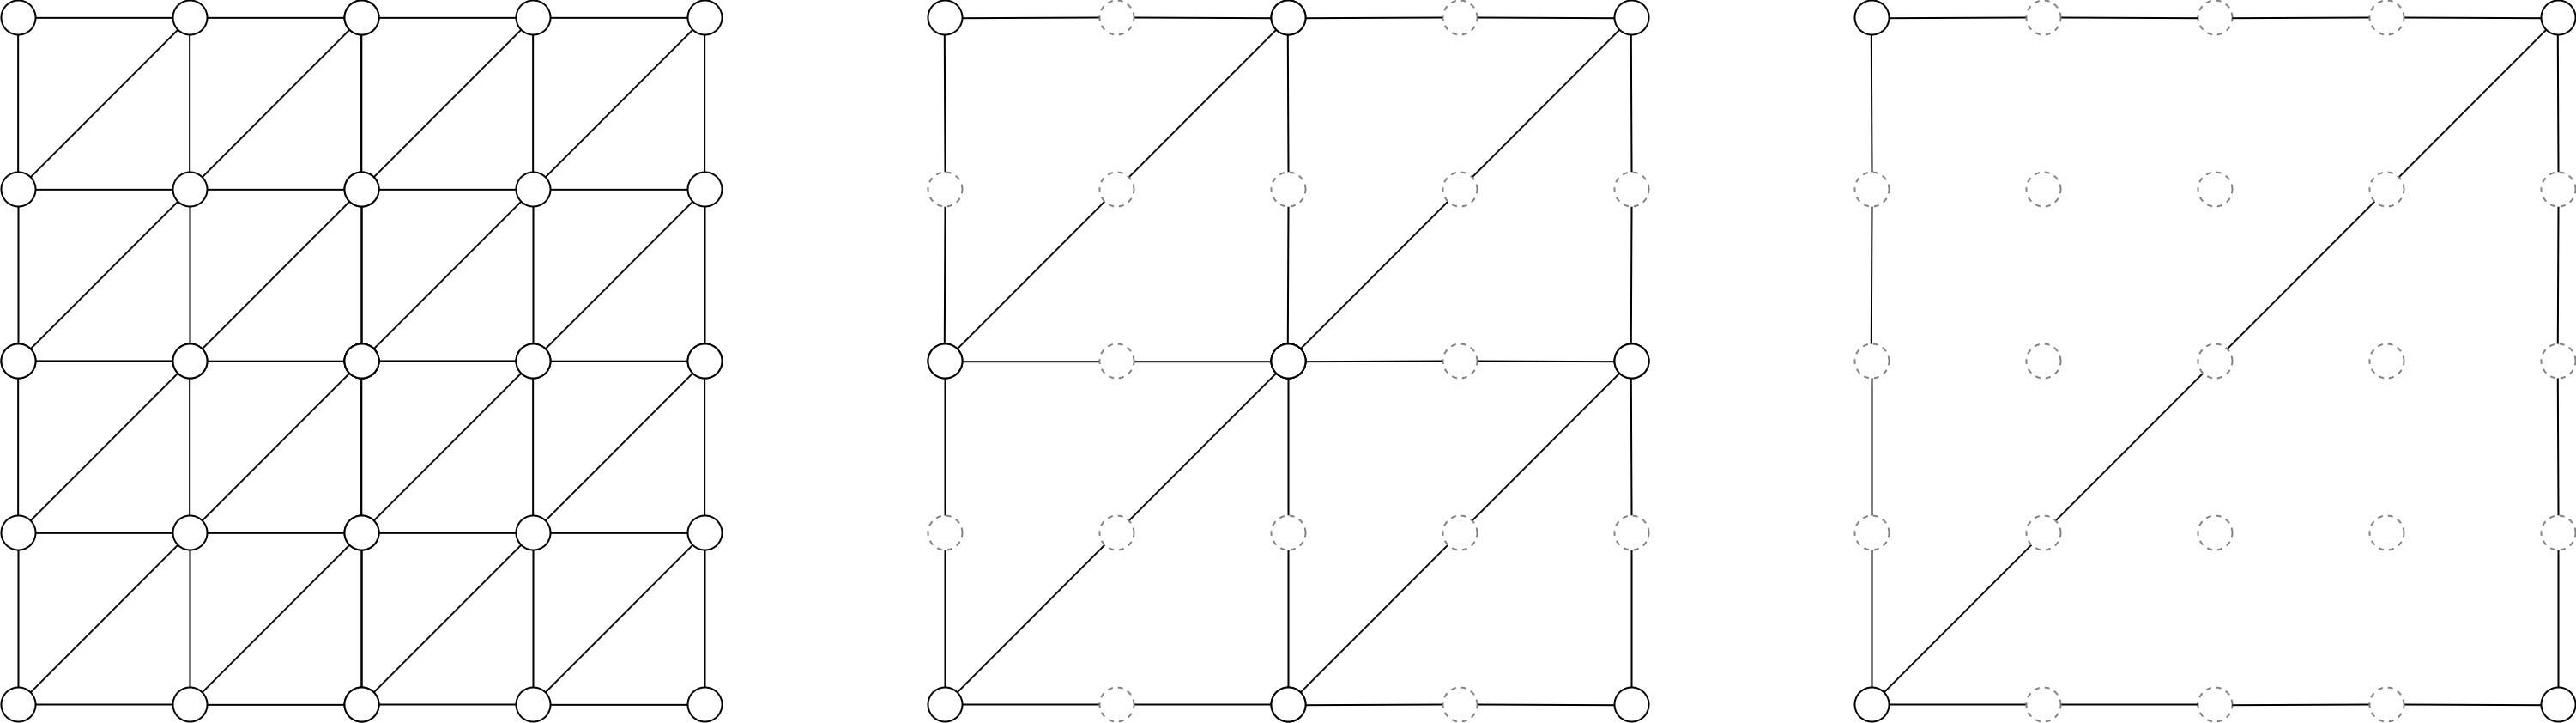
\includegraphics[width=1\textwidth]{geomipmapping-patch-example}
%   \caption{Example of a $5 \times 5$ block at the maximum LOD level of 2 (left), LOD level of 1 (middle) and minimum LOD level of 0 (right). The omitted vertices of the lower LOD blocks are shown here as dotted circles.}\label{fig:geomipmapping-patch-example}
% \end{figure}

\begin{figure}[H]
  \centering
  \subfloat[\centering LOD level 2 (maximum).]{{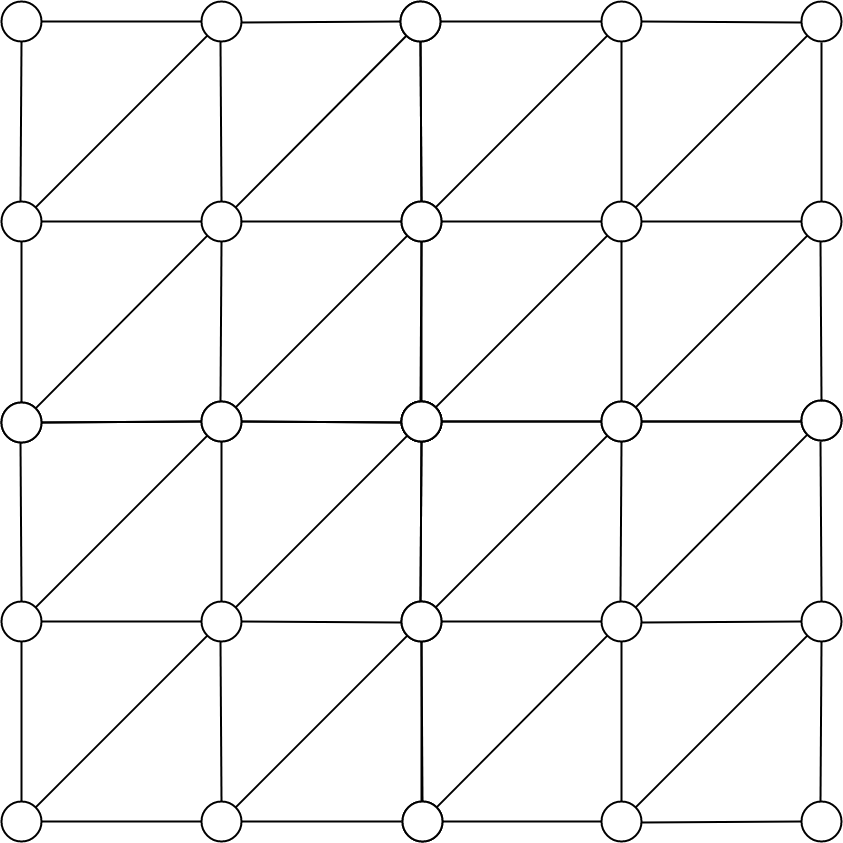
\includegraphics[width=0.28\textwidth]{geomipmapping-level-2.png} }}
  \qquad
  \subfloat[\centering LOD level 1.]{{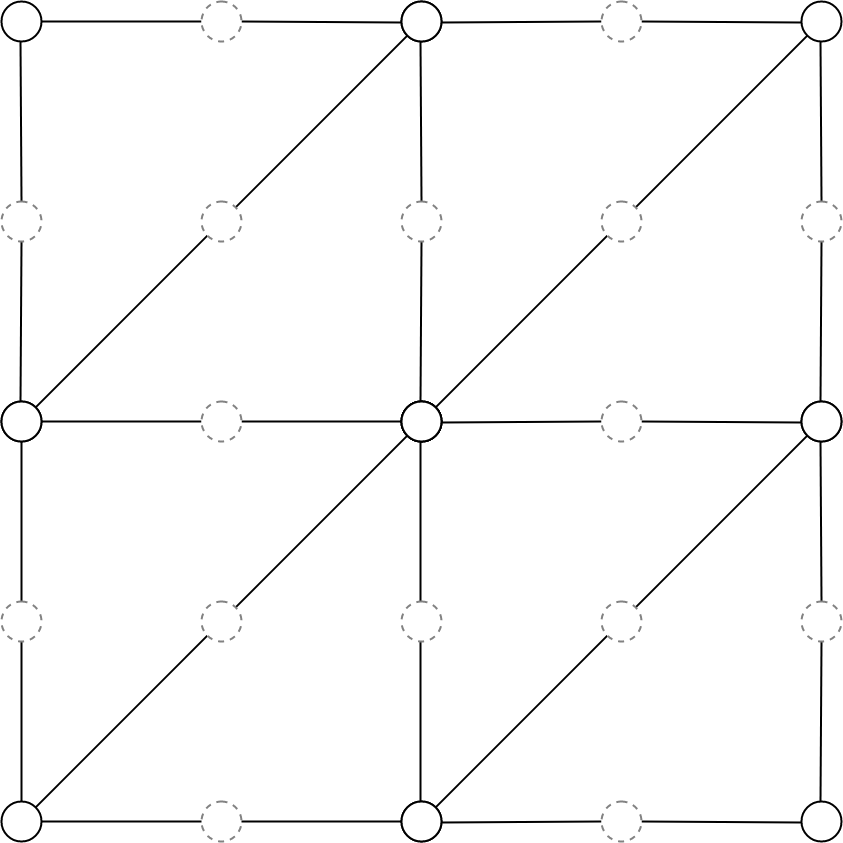
\includegraphics[width=0.28\textwidth]{geomipmapping-level-1.png} }}
  \qquad
  \subfloat[\centering LOD level 0 (minimum).]{{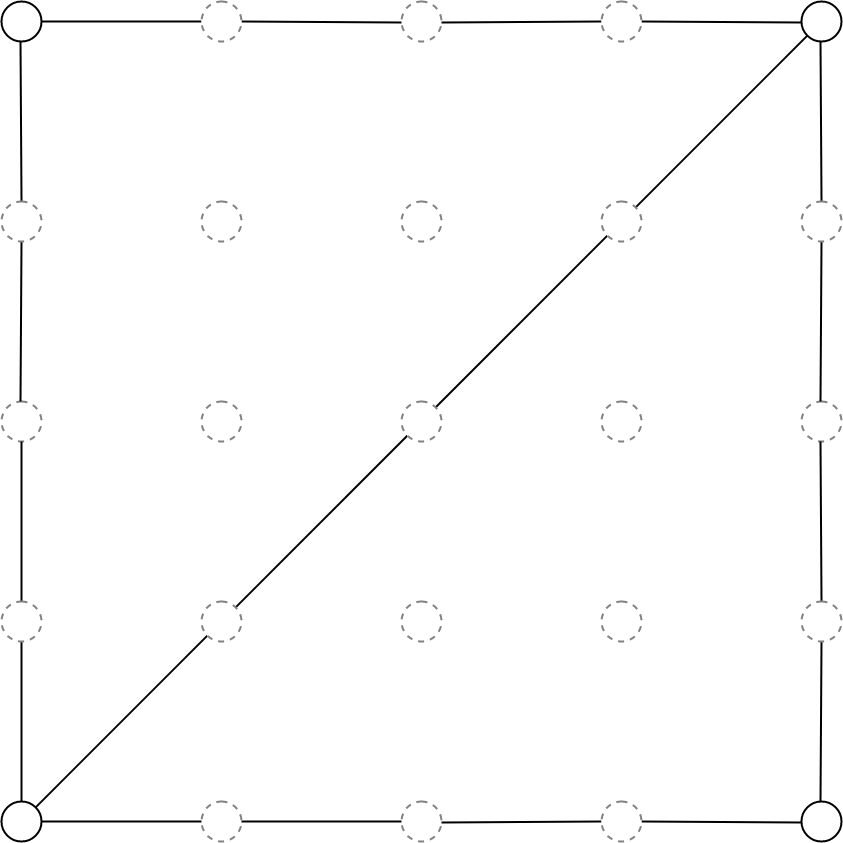
\includegraphics[width=0.28\textwidth]{geomipmapping-level-0.png} }}
  \caption{Example of each GeoMipMap of a $5 \times 5$ block. The omitted vertices of lower LOD GeoMipMaps are marked as dotted circles.}\label{fig:geomipmapping-patch-example}
\end{figure}

\subsection{Avoiding Cracks}
GeoMipMapping avoids cracks in the terrain by first checking whether the
current block has a higher LOD than the bordering block.
If this is the case, then the edge that causes the crack 
needs to not get drawn. This is done by rendering the border area between two blocks
as triangle fans, as shown in figure~\ref{fig:geomipmapping-crack-avoidance}.

\begin{figure}[H]
  \centering
  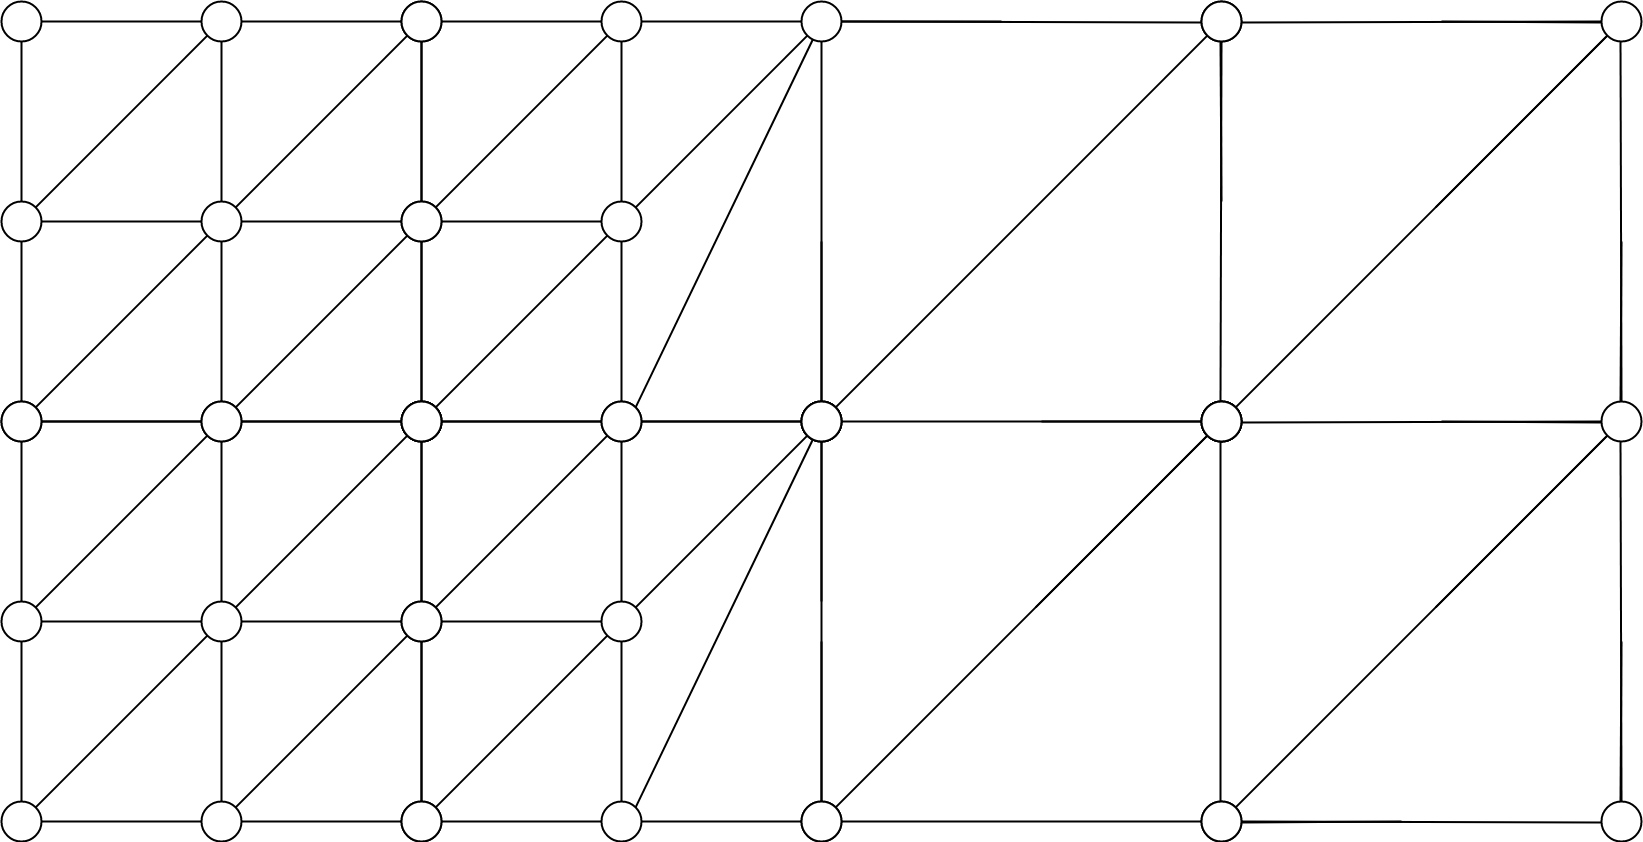
\includegraphics[width=0.7\textwidth]{geomipmapping-crack-avoidance}
  \caption{Example of GeoMipMapping's crack avoidance between a LOD 2 and a LOD 1 GeoMipMap of two $5 \times 5$ blocks.}\label{fig:geomipmapping-crack-avoidance}
\end{figure}

This means that the LOD levels of the neighboring blocks need to be stored in a structure on each block.
This structure is updated continually at runtime.

\subsection{LOD Selection}

\subsection{Other Optimizations}
\paragraph{Vertex Morphing}
GeoMipMapping can be extended with vertex morphing in order to decrease popping.

\paragraph{View-frustum Culling}
Blocks that are outside of the view-frustum can be left out completely, thereby dramatically decreasing the number 
of vertices that need to get rendered.
The GeoMipMapping paper mentions using quadtrees to  


\section{Geometry Clipmaps}
TODO

%\section{CDLOD}
%TODO

